\documentclass[9pt, oneside]{extarticle}   	% use "amsart" instead of "article" for AMSLaTeX format
%\documentclass[9pt,twocolumn,oneside]{extarticle}   	% use for two column
\usepackage{graphicx}				% Use pdf, png, jpg, or eps� with pdflatex; use eps in DVI mode
								% TeX will automatically convert eps --> pdf in pdflatex								
\usepackage[margin=2cm]{geometry}
\usepackage{amssymb}
\usepackage{tikz,adjust box}			%adjustbox is for figures that span 2 columns
\usepackage{dashrule}				%used to make dashed line in text
\usepackage{amsmath}
\usepackage{multicol}
\usepackage{fancyhdr}				%used to put draft in header
\DeclareMathOperator{\arcsec}{arcsec}	%arcsec, arccsc... not defined inamsmath
\usepackage{exsheets}				%Formats questions and solutions
\SetupExSheets{solution/print=false,question/name={},solution/name={}}		%Solutions on or off; 
\SetupExSheets{headings=runin}		% Puts questions next to number
\SetupExSheets{use-classes={easy,medium,hard}}	% Print questions by difficulty level
\usepackage{natbib,endnotes}			%Bibliography and Footnote to endnote

\usepackage{title sec}				%Format section titles to include horizontal line
\usepackage{enumitem}				%Allow lists to be a, b, c and not 1, 2, 3

\setenumerate[0]{label=(\alph*)}
%\let\footnote=\endnote
\titleformat{\section}
  {\normalfont\Large\bfseries}{\thesection}{1em}{}[{\titlerule[0.8pt]}]
\newcommand{\calc}{\protect\includegraphics[height = 2.5ex]{images/calc.png}}  

\newcommand{\thedate}{8/27/2014}
\newcommand{\theexam}{Notes \S 1.6 Rates}
\newcommand{\thecourse}{PreCalculus $\infty$ Briody}

%%%%%%Macros: begin question cntrl command Q or S for solution
\title{Problem Solving}
\author{PHS}
\date{today}							% Activate to display a given date or no date
%\chead{draft\_draft\_draft\_draft\_draft\_draft}
\begin{document}
\pagestyle{fancy}
\lhead{\thecourse} \chead{\theexam} \rhead{\thedate}
\lfoot{} \cfoot{\thepage} \rfoot{}
\renewcommand{\headrulewidth}{0.4pt} \renewcommand{\footrulewidth}{0.4pt}
\thispagestyle{plain}

\parindent 0ex
\textbf{\thecourse} \hfill  \textbf{Name:}
\makebox[6cm]{\hrulefill}

\textbf{\theexam} \hfill \textbf{\thedate}
\rule[1ex]{\textwidth}{.1pt}
{\large {\bf Objectives} You should be able to:
\begin{itemize}
\item find distance, time or rate given two of the three
\item find rate from a distance vs. time graph
\item know the difference between {\bf speed} and {\bf velocity}
\item extract information from a velocity vs. time graph
\end{itemize}
\hrule 
\kern3pt
%\section{Functions}
%\input{subsections/func} 
\begin{question}[class=easy]
John leaves home at 8:00 A.M. riding his mountain bike. He pedals at a constant rate of 15 ft/s. 
\begin{enumerate}
\item How far has John ridden at 8:10 A.M.?
\item How far has John ridden at 8:20 A.M.?
\item How far has John ridden at 8:45 A.M.?
\item Write an expression for how far John has ridden $t$ minutes after 8:00 A.M.
\end{enumerate}
\end{question}
\begin{solution}
\begin{enumerate}
\item 9000 ft or approx. 1.7mi
\item 18000 ft or approx. 3.4mi
\item 40,500 ft or approx. 7.7mi
\item 900$t$ ft
\end{enumerate}� \cite[p.186]{Project2008}
\end{solution}

\begin{question}[class=easy]
Pete, John's older brother, leaves 10 minutes after John, heading down the sam trail. He rides at 20 ft/sec.
\begin{enumerate}
\item How far has Pete ridden at 8:10 A.M.? Has Pete caught John?
\item How far has Pete ridden at 8:20 A.M.? Has Pete caught John?
\item How far has Pete ridden at 8:45 A.M.? Has Pete caught John?
\item Write an expression for how far Pete has ridden at $t$ minutes after 8:00 A.M.
\item How can you find the exact time Pete caught John?
\end{enumerate}
\end{question}
\begin{solution}
\begin{enumerate}
\item 0 ft; Pete has not caught John
\item 1200 ft or 2.25mi; Pete has not caught John
\item 42,000 ft or about 8 mi; Pete has passed John
\item $1200(t-10)$, where $t\geq$10
\item Solve $900t=1200(t-10)$
\end{enumerate}�
 \cite[p.186]{Project2008}
\end{solution}

\begin{question}[class=easy]
Demitri and Yakov are running on a track. The figure below shows their distance-time graphs.\\
%%%%%%%%%%coordinate plane with function%%%%%%%%%
%\begin{tikzpicture}[scale=.2]
\begin{tikzpicture}[y=.05cm, x=.5cm]
\draw[style=help lines, ystep=10, xstep=1] (0,0) grid
  (10,60);
\draw[thick,-] (0,0) -- coordinate (x axis mid) (10,0);% node[anchor=south east] {$x$};
\draw[thick,-] (0,0) -- coordinate (y axis mid) (0,60);% node[anchor=north west] {$y$};
\foreach \x in {0,2,4,6,8,10}
    \draw (\x ,1pt) -- (\x ,-1pt) node[anchor=north] {$\x$};
\foreach \y in {0,20,40,60}
    \draw (1pt,\y ) -- (-1pt,\y ) node[anchor=east] {$\y$};
%\draw[<->, ultra thick, domain=-1.3:7.15,smooth] plot (\x, {-1*(\x+1)*(\x-4)*(\x-6)});
\draw[-, ultra thick, domain=-0:6,smooth] plot (\x, {10*\x}); %node[rotate=45,anchor=south east] {$Y$};
\node[rotate=45] at (4,45) {Yakov};
\node[rotate=0] at (7,35) {Demitri};
\draw[-, ultra thick, domain=-0:10,smooth] plot (\x, {5*\x+10}); %node[anchor=south east] {$D$};
\node[below=0.8cm] at (x axis mid) {Time (seconds)};
\node[rotate=90, above=0.8cm] at (y axis mid) {Distance (feet)};
\end{tikzpicture}\\
%%%%%%%%%%%%%%%%%%%%%%%%%%
\begin{enumerate}
\item Who is running faster, Demitri or Yakov?
\item When does Yakov overtake Demitri?
\item At what distance does Yakov overtake Demitri?
\item What is each runner's speed?
\item Write an equation for Yakov's graph.
\item Write an equation for Demitri's graph.
\item Write and solve an equation for which the solution is the time at which Yakov overtakes Demitri.
\end{enumerate}
\end{question}
\begin{solution}
\begin{enumerate}
\item Yakov
\item 2 s
\item 20 ft
\item Yakov: 10 ft/s; Demitri: 5 ft/s
\item $y=10x$
\item $y=5x+10$
\item $10x=5x+10$
\end{enumerate}�
 \cite[p. 186]{Project2008}
\end{solution}

\begin{question}[class=medium]
Suppose that $a$ cows give $b$ gallons of milk in $c$ days. At this rate, how many gallons of milk will $d$ cows give in $e$ days?
\end{question}
\begin{solution}
$\frac{bde}{ac}$ \cite[\#4]{AHSME2014}
\end{solution}

\begin{question}[class=medium]
Toby drives exactly 200 miles from San Jose to Morro Bay, CA. The trip takes exactly four hours. Show that at some point in the trip, Tony's speedometer indicates a speed of exactly 50 miies per hour.
\end{question}
\begin{solution}
Average speed was $\frac{200}{4}=50$ miles per hour and by IVT if there is a time $t_{1}$ where he is going less than 50 mph and a time $t_{2}$ where he is going more than 50 mph there must be a time where he is going exactly 50 mph. \cite[p.177]{Project2008}
\end{solution}

\begin{question}[class=medium]
In parts \ref{MOA} and \ref{MOB}, use the velocity/time graph to answer the questions. Assume that North is positive and South is negative. Time is measured in hours and velocity in miles per hour. You start your journey from home at noon\footnote{We know it is unrealistic to instantly change from $0mph$ to $-30mph$ at 0 hours. Calculus addresses this situation.}.

\begin{centering}
%%%%%%%%%%GRAPH%%%%%%%%%%%%%
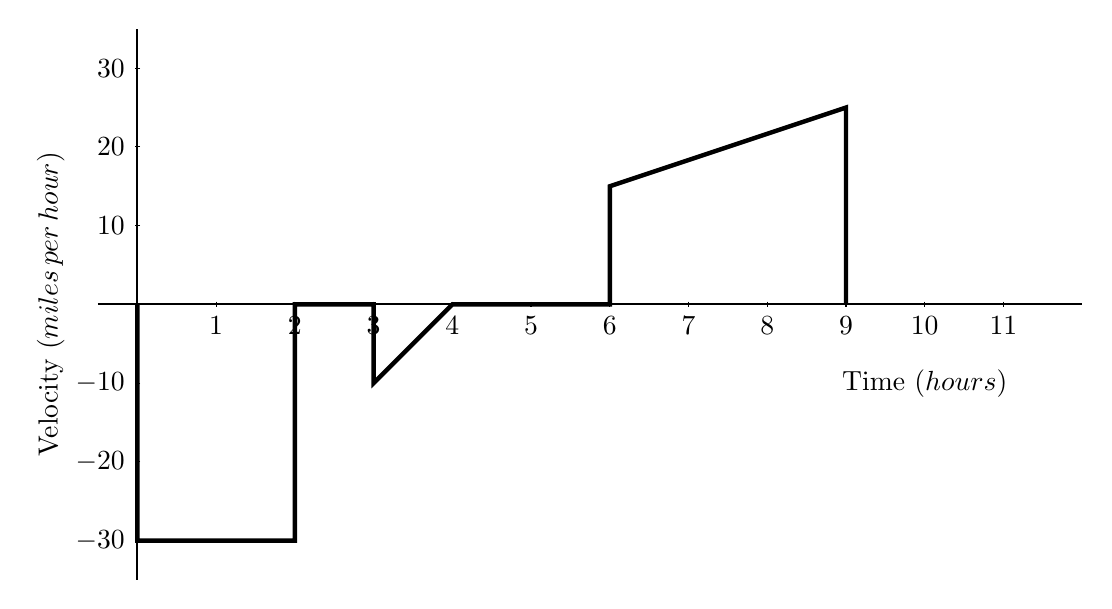
\begin{tikzpicture}[y=.1cm, x=1cm]
%\draw[style=help lines, ystep=5, xstep=1] (-2,-35) grid  (12,35);
\draw[thick,-] (-.5,0) -- coordinate (x axis mid) (12,0); %node[anchor=north west] {$x$};
\draw[thick,-] (0,-35) -- coordinate (y axis mid) (0,35);% node[anchor=north west] {$y$};
\foreach \x in {1,2,3,4,5,6,7,8,9,10,11}
    \draw (\x ,1pt) -- (\x ,-1pt) node[anchor=north] {$\x$};
\foreach \y in {-30, -20, -10, 10, 20, 30}
    \draw (1pt,\y ) -- (-1pt,\y ) node[anchor=east] {$\y$};
\node at (10,-10) {Time ($hours$)};
\draw[ultra thick,-] (0,0)--(0,-30)--(2,-30)--(2,0)--(3,0)--(3,-10)--(4,0)--(6,0)--(6,15)--(9,25)--(9,0);
\node[rotate=90, above=0.8cm] at (y axis mid) {Velocity ($miles\, per\, hour$)};
\end{tikzpicture}\\
%%%%%%%%%%GRAPH%%%%%%%%%%%%%
\end{centering}
\begin{enumerate}
\item \label{MOA} Approximately how many miles would your odometer say you drove between noon and 3PM?
\item \label{MOB} Approximately how many miles would your odometer say you drove between 3PM and 6PM?
\item Approximately how many miles would your odometer say you drove between 6PM and 9PM?
\item Approximately how many miles from home did you end up?
\item \calc\ At 7PM, approximately how far from home are you?
\item If $speed=|velocity|$, sketch your speed on the graph using a dashed \mbox{(\hdashrule[0.5ex]{1.5cm}{1pt}{1mm})} line.
\item When is your velocity...
\begin{enumerate}[label=\roman*]
\item constant?
\item increasing?
\item decreasing?
\end{enumerate}� 
Please use interval notation
\end{enumerate}�
\end{question}
\begin{solution}
\begin{enumerate}
\item 60 miles
\item 5 miles
\item 60 miles
\item $v-15=\frac{10}{3}(t-6)$\\ $60S +5S-.5[(\frac{10}{3}(7-6)+15)+15]*1N=48.333$ miles
\item Reflect all negative velocities across the time axis to make them positive.\\
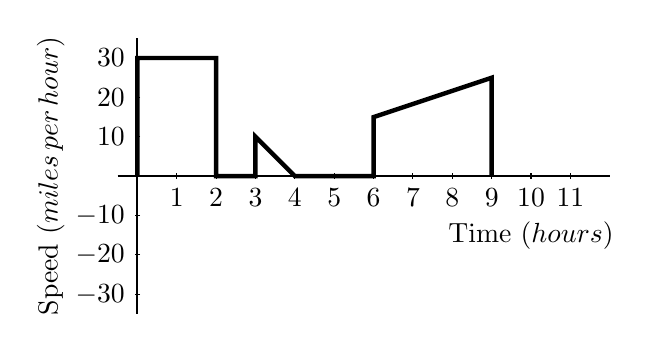
\begin{tikzpicture}[y=.05cm, x=.5cm]
%\draw[style=help lines, ystep=5, xstep=1] (-2,-35) grid  (12,35);
\draw[thick,-] (-.5,0) -- coordinate (x axis mid) (12,0); %node[anchor=north west] {$x$};
\draw[thick,-] (0,-35) -- coordinate (y axis mid) (0,35);% node[anchor=north west] {$y$};
\foreach \x in {1,2,3,4,5,6,7,8,9,10,11}
    \draw (\x ,1pt) -- (\x ,-1pt) node[anchor=north] {$\x$};
\foreach \y in {-30, -20, -10, 10, 20, 30}
    \draw (1pt,\y ) -- (-1pt,\y ) node[anchor=east] {$\y$};
\node at (10,-15) {Time ($hours$)};
\draw[ultra thick,-] (0,0)--(0,30)--(2,30)--(2,0)--(3,0)--(3,10)--(4,0)--(6,0)--(6,15)--(9,25)--(9,0);
\node[rotate=90, above=0.8cm] at (y axis mid) {Speed ($miles\, per\, hour$)};
\end{tikzpicture}\\
\item 
\begin{enumerate}[label=\roman*]
\item $(0,2),(2,3),(4,6)$ hours
\item $(6,9)$ hours
\item $(3,4)$ hours
\end{enumerate} 
\end{enumerate}� \cite[p. 1]{Mauer-Oats}
\end{solution}
\hrule
%%%%%%%%%%%Homework%%%%%%%
{\bf Homework:}
\setcounter{question}{0}
\begin{question}[class=medium]
Book: p. \# 100-212\\
\end{question}
\begin{solution}
Answers \cite[]{cohen}
\end{solution}
\begin{question}[class=medium]
Given two functions: $w(x)=\frac{1}{x^{2}}$  
\end{question}
\begin{solution}
 solution\cite[p. 7]{Mauer-Oats}
\end{solution}
\newpage
\begin{multicols}{2}
\section{SOLUTIONS}
\printsolutions
\bibliographystyle{te}
\bibliography{temp}
\end{multicols}
\vfill
\bf{More Velocity vs Time graph questions in conference packet.}
%\theendnotes
\end{document}